\subsection{One physical hop strengthens the unchanged Li6 source}
\label{sec:li6-one-hop-12}

The next verified trial keeps the Hamiltonian
\eqref{eq:scalar-law-new}, the source600 metric, phase 9, unchanged address
14336 and $(\tau,t_c,g^2)=(1,10^{-3},35)$. Let $J_\lambda$ be its
cloud-dressed target map in the orbital sectors $\lambda=42,33,321$.
For the physical off-diagonal hopping $K$, write
$V_\lambda=J_\lambda^*K^2J_\lambda$. The graph-polar map is
\begin{equation}
 J_{\lambda,\alpha}
 =(J_\lambda-\alpha_\lambda KJ_\lambda)
       (I+\alpha_\lambda^2V_\lambda)^{-1/2},
\label{eq:one-hop-polar-12}
\end{equation}
with $\alpha_{42}=\alpha_{33}=1/56$ and $\alpha_{321}=1/40$.
Parity removes the target/one-hop norm cross term. All internal and cell
hops, coherent-cloud overlaps, field self energy and both ordered vertex
terms remain in the energy compression. The normalization is a full
matrix congruence, rather than a columnwise normalization.
\samref{REF12_CAR}

The separately rebuilt compression lowers the unchanged-source energy
upper by more than $1.0501207340$, so its margin against the same
$-728/3$ proper-fragment lower is
\begin{equation}
 m_\alpha>1.6027627093.
\label{eq:li6-one-hop-margin-12}
\end{equation}
For the entire stated real passive harmonic family with the same static
$G$, each receiver's own coherent clouds give gain greater than
$0.7603001617$ and margin greater than $1.3129421370$. These are
alternative full-Fock preparations under their stated laws. They do not
add to the earlier loading, clock or calibration allowances.

The orbital construction extends to a common full-parent isometry and
transports every original Write. Its favorable mean-energy upper applies
to the unchanged 14336 preparation, not to every source600 vector. A
pure-$411$ control breaks that stronger assertion. Similarly the sufficient
sector uppers put $42$ and $33$ more than $31.6161863519$ and
$16.1415545876$ below the common proper lower, while the $321$ upper is
$20.8492111446$ above it. An upper above a threshold does not establish a
ground-state lower above that threshold. The weighted source certificate
therefore supplies no all-sector stable-band conclusion.

\begin{figure}[htbp]\centering
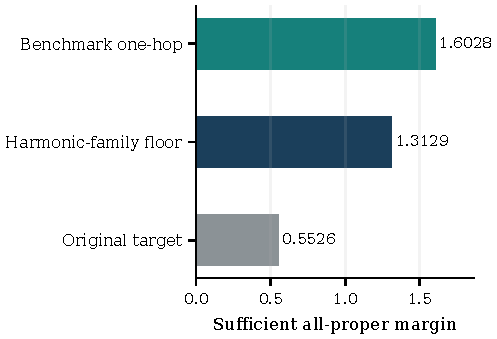
\includegraphics[width=\columnwidth]{refinement_20261112/figures/li6_margins.pdf}
\caption{Sufficient margins for the same unchanged Li6 source. Each bar
is its own complete energy comparison. The harmonic-family bar is a
uniform lower guarantee with each law's own field dressing.}
\label{fig:li6-margins-12}
\end{figure}

\subsection{A source-connected twelve-particle all-proper certificate}
\label{sec:n12-12}

A new construction starts from two already prepared contact Li6 sources
in distinct cells. It has flavor populations $(4,2,4,2)$ and inventory
$6p6n$. This route differs from the earlier three-He4 carbon preparation;
the inventory alone does not identify the preparation or its cost.
The one-cell fixed-weight CAR parent has dimension $3{,}841{,}600$.
Under the unchanged counterterm-free scalar law, enumeration of all
$5^8=390{,}625$ site occupancies, network-flow/Gale--Ryser capacity cuts
and dynamic programming over all 225 flavor subvectors bounds every
proper fragment. There are 223 nontrivial ordered binary flavor splits.
Refining a many-fragment split cannot evade the complete binary bound.
The worst static numerator is 2340 at $11+1$, giving
\begin{equation}
 L_{{\rm proper},12}\ge-780\qquad(g^2=35).
\end{equation}
This is an all-cell, all-proper matter/flavor lower with the same full
Fock completion, not a test of only the selected dissociation channel.

Among the 420 even-occupancy $(4,4,2,2,0,0,0,0)$ Slaters, choose 25 in
the $U(4)$ Casimir-48 highest-weight irrep. Single-hop matrix elements
within this selected family vanish. The full flavor fiber has dimension
36 and central ranks $1,15,20$; 25 complete 20-dimensional orbital copies
retain the actual source action. Their static numerator is at least
$2592/105$. Consequently
\begin{align}
 U_{25}&\le-98991/125=-791.928,\\
 L_{{\rm proper},12}-U_{25}&\ge1491/125=11.928.
\label{eq:n12-margin-12}
\end{align}
More generally the sufficient margin is
$(12/5)g^2-72(\tau+t_c)$, positive when
$g^2>30(\tau+t_c)$.\samref{REF12_CAR}

The unchanged incoming pair succeeds with exact probability
$28561/455625$. Its 81-dimensional source has success rank 25 and a
failure operator of rank 80; these ranks refer to operators with a common
source domain, not an orthogonal partition of that domain. A coherent
retained outcome flag transports the full Gram and Writes. The energy
certificate is conditional on success. The supplied bare-target/free-vacuum
discrete loading example has allowance $25411/12500=2.03288$ at
$\mathcal A\le1/200$. It does not pay for incoming clouds, projection,
arrival control or reusable reset. The alternative external-cell-record
receiver has margin $9473/375$ and is a changed receiver. Neither the
one-cell matter capacity nor its prescribed equilibrium dressing is a
capacity bound on unrestricted Fock memory.

\subsection{Translation fibers, escaped bosons and two isolated bands}
\label{sec:fiber-12}

The refinement supplies the spectral argument that the preceding
mean-energy comparison alone did not contain. Its hypotheses are exactly
the benchmark lattice law: fixed six fermions, four flavors, finite-range
density vertex, no intercell boson propagation and optical frequencies
$1,3,5,7$. Simultaneous cell translations act freely on finite matter
configurations and commute with flavor. Fourier transformation of their
orbits gives
\begin{equation}
 H=\int_{\mathbb T^3}^{\oplus}H(P)\,\frac{\dd P}{(2\pi)^3},
 \qquad E_\lambda(P)=\inf\sigma H_\lambda(P).
\end{equation}
The domains are the full $D(N_b)$ and form domains $D(N_b^{1/2})$;
Young's inequality gives $H(P)\ge N_b/2-C_{N,g}$ uniformly. Only matter
cell hopping twists with $P$. Its row/column sum bounds the band width by
$12Nt_c=72t_c$. A center-of-mass phase intertwiner establishes local
norm continuity of the twisted hopping, so $E_\lambda$ is continuous and
$e_\lambda=\min_QE_\lambda(Q)$ exists.\samref{REF12_ONE}

For completeness, the localization proof retains the order of limits.
First cut off boson number smoothly at $2M$. The vertex changes number by
one, giving commutator norm $O(M^{-1/2})$ and energy-bounded tail mass
$O(M^{-1})$. At fixed $M$, a translation-invariant matter partition of
unity separates every proper cluster configuration at scale $R$.
Antisymmetric cluster tensor maps retain all flavor allocations. A field
partition $j_a,j_\infty$ equals one at the corresponding occupied matter
cells and has Lipschitz constant $O(R^{-1})$. Because the frequencies act
only within cells, $[\omega,j_a]=0$ exactly and the density vertex
intertwines into the appropriate cluster without error. Matter hopping
changes the Fock partition by at most $O(M/R)$, so the complete
intertwining defect is $O(t_c(1+M)/R)$.

A proper matter branch is bounded by $L_{\rm proper}$. On the single
matter cluster with a remote boson, the comparison is at least
$e_\lambda+1$. With no remote boson and fixed $M,R$, the relative lattice
coordinates and boson occupations form a finite-rank space in a fixed
fiber. It disappears on a weakly null Weyl sequence. Take the Weyl-sequence
limit first, then $R\to\infty$, then $M\to\infty$. This proves
\begin{equation}
 \inf\sigma_{\rm ess}H_\lambda(P)
 \ge\min\{L_{\rm proper},e_\lambda+1\}.
\label{eq:fiber-threshold-12}
\end{equation}
The free-boson branch is essential even when matter breakup lies much
higher. No finite photon cutoff defines the assertion.

Translated one-hop targets have no cross-center norm or energy matrix
elements: these use at most two or three hops, whereas translating all
six matter particles requires six cell hops. The finite path control is
zero after three hops and 720 after six. Thus the same sector trial upper
holds in every fiber. Combining the $42,33$ proper margins with
$E_\lambda(P)-e_\lambda\le72t_c=9/125$ gives
\begin{equation}
 \inf\sigma_{\rm ess}H_\lambda(P)-E_\lambda(P)
 \ge116/125=0.928,\qquad\lambda=42,33.
\label{eq:fiber-gap-12}
\end{equation}
Their bottoms are isolated finite-multiplicity eigenvalues, including the
finite flavor factors. This analytical lattice theorem has native finite
kinematic anchors; it is not a new independent CR2 certification of the
infinite-dimensional argument. It supplies no $321$ conclusion, prepared
released eigenstate, lifetime, capture amplitude or electromagnetic
nuclear prediction.
